\documentclass[a4paper,11pt, titlepage]{article}

\usepackage[left=20mm, text={170mm, 240mm}, top=30mm]{geometry}
\usepackage[czech]{babel}
\usepackage[IL2]{fontenc}
\usepackage[utf8x]{inputenc}
\usepackage{enumitem}
\usepackage{scrextend}
\usepackage{lscape}
\usepackage{times}
\usepackage{graphicx}
\usepackage[T1]{fontenc}
\usepackage{lmodern}
\usepackage{indentfirst}

\usepackage{mathtools}
\usepackage{amsfonts}
\usepackage{amsthm}

\setlength{\parskip}{1em}

\begin{document}

\begin{titlepage}
	
	\begin{center}
		{\Huge\textsc{Vysoké učení technické v~Brně}}\\
		\medskip
		{\huge\textsc{Fakulta informačních technologií}}\\
		\vspace{\stretch{0.382}}
		{\huge Hamiltonova cesta a cyklus v grafe}\\
		\medskip
		{\LARGE Náhradný projekt IAL}\\
		\vspace{\stretch{0.618}}
	\end{center}
	
		
	
	
	\Large {\hfill Brno, \today}
	
\end{titlepage}

\section{Úvod}

Dokumentácia popisuje návrh a~implementáciu riešenia projektu hamiltonovej cesty a~cyklu v~hamiltonovom grafe. Súčasťou je aj porovnanie teoretickej zložitosti úlohy a experimentálnych výsledkov nášho riešenia.

\section{Analýza problému}

\subsection{Hamiltonovský graf a cesta}

Hamiltonovský graf \cite{Wikipedia_Hamilton_Path} je taký graf, ktorý je možné prepojiť takou cestou, že každý jeho uzol je navštívený práve raz s výnimkou uzlu počiatočného, ktorý je zároveň uzlom cieľovým. Inak povedané, graf je hamiltonovský, práve keď obsahuje kružnicu, ktorá prechádza všetkými jeho uzlami, pričom žiadnym uzlom neprechádza viac ako raz (ide o tzv. hamiltonovskú kružnicu, resp. hamiltonovský cyklus) \cite{Studijni_opora}.

\begin{figure}[h]
\centering
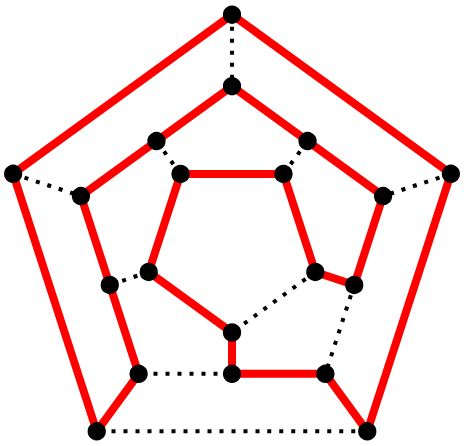
\includegraphics[scale=0.25]{path.JPG}
\caption{Hamiltonova kružnica}
\label{Obr. 1}
\end{figure}

\par
Hamiltonovská cesta \cite{EU} je taká cesta v danom grafe, ktorá prechádza každým jeho vrcholom práve raz. Každý graf však nemusí mať nutne hamiltonovskú kružnicu. Nutnými (ale nie postačujúcimi) podmienkami sú, že graf musí byť súvislý a každý vrchol musí mať stupeň rovný najmenej dvom (ku každému vrcholu musia viesť aspoň dve hrany). Problém nachádzania hamiltonovskej kružnice je NP-úplný, napr. problém obchodného cestujúceho (tj. nájdenie najkratšej hamiltonovskej kružnice). NP znamená riešitelný nedeterministicky v~polyniomiálnom čase. Ľubovolný NP problém je možné v~polynomiálnom čase previesť na NP-úplný.

\begin{figure}[h]
\centering
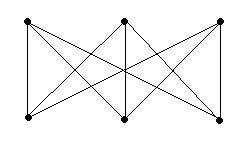
\includegraphics[scale=0.75]{hamiltcycle.JPG}
\caption{Hamiltonova cesta a cyklus (znázornenie)}
\label{Obr. 2}
\end{figure}

\par
Aj keď sa hamiltonovské grafy zdajú byť obdobou eulerovských grafov \cite{SFU}, rozhodnúť, či je graf hamiltonovský, nie je vždy jednoduché. Známych je však niekoľko podmienok, na základe ktorých môžeme rozhodnúť či ide o graf hamiltonovský alebo nie.
Na obrázku č.3 vidíme znázornenú Hamiltonovu cestu. Nie každý graf nutne musí obsahovať kružnicu (cyklus). V tomto prípade je počiatočný a koncový bod rozdielny.

\begin{figure}[h]
\centering
\includegraphics[scale=0.75]{ham_cesta.JPG}
\caption{Hamiltonova cesta}
\label{Obr. 3}
\end{figure}

\subsubsection{Podmienky pre hamiltonovský graf}
\par
$V$ je počet uzlov grafu. Predpokladajme, že $V \geq 3$. K tomu, aby bol graf hamiltonovský, teda stačí splnenie niektorej z nasledujúcich podmienok:

\begin{itemize}[noitemsep]
	\item Ak má každý stupeň aspoň \(\frac{1}{2}\) $V$, graf je hamiltonovský (Diracova podmienka).\vspace{0.25cm}
	\item Ak pre každú dvojicu uzlov, ktoré nie sú spojené hranou, súčet ich stupňov je aspoň $V$, potom je graf hamiltonovský (Oreho podmienka). \vspace{0.25cm}
	\item Ak pre každé prirodzené číslo $k < \frac{1}{2} V$ je počet uzlov, ktorých stupeň neprevyšuje $k$, menšie než~$k$, potom je graf hamiltonovský (Pósova podmienka).
\end{itemize}

\section{Implementácia riešenia}

Prvým krokom pri riešení projektu bolo nastavenie potrebných vyššie uvedených podmienok, kedy sme zisťovali, či testovaný graf je hamiltonovským grafom (resp. cyklom), či existuje hamiltonovská cesta alebo nie. V prípade, že áno, začneme hľadať všetky jeho riešenia. V prípade, že tento graf (resp. cyklus) nie je hamiltonovský, riešenie neexistuje, a teda sa na výstupe objaví chybové hlásenie.

\subsection{Program}

Zadanie sme sa rozhodli riešiť metódou "brute force", kde každý uzol má oddelené vlákno, funkcie sa volajú rekurzívne a v oddelených vláknach pokračuje grafom. Pamätáme si akými vrcholmi sme už prešli. Pokiaľ vlákno nájde koncový bod a prešlo už všetky body, tak za pomoci semaforu vypíše výsledok na výstup (jedná sa o viacriadkový výpis). Vlákno končí bez výpisu Hamiltonovej cesty pokiaľ sa dostane do bodu, odkiaľ nemôže pokračovať ďalej bez toho, aby nejaký vrchol navštívilo viac než raz. Dáta programu sú ukladané do dátových štruktúr.

\subsection{Testovanie a ladenie} 

Jeden vstupný graf zodpovedá jednému vstupnému súboru. Každý súbor v zložke \texttt{tests/params\_in} zodpovedá jednému grafu a obsahuje po riadkoch rôzne sady spúšťajúcich parametrov. Pre zjednodušenie práce sú hrany vo vstupnom súbore radené vždy podľa abecedy a~podľa abecedy sú radené i~vrcholy jednotlivých hrán. To isté platí u referenčného výstupu, a teda i očakávaného výstupu programu. Všetky testovacie grafy sú umiestnené v zložke \texttt{tests/graph\_in}, ich referenčný výstup je v~zložke \texttt{tests/ref\_paths\_out}. 

\par
Príkazom \emph{make test} v koreňovom adresári dôjde k spusteniu programu so všetkými dostupnými grafmi a postupne so všetkými ich parametrami, uloženie ich výstupu do \texttt{test/output} a porovnávanie s referenčným výstupom (výstup z porovnania je v zložke \texttt{test/diff}). Pokiaľ je očakávaný návratový kód u danej varianty grafu (teda napr. graf 1 s 2. sadou parametrov: 1.2) rôzny od nuly, je treba vytvoriť referenčný súbor s návratovým kódom v zložke(\texttt{tests/ref\_paths\_out}) v tvare \texttt{graf.parametry.rc} (teda napr. \texttt{1.2.rc}), kde obsahom súboru je na prvom riadku očakávaný návratový kód.

\subsection{Spustenie programu}

\subsubsection{Ukážka spustenia manuálne z príkazového riadku}

\includegraphics[]{manual.JPG}

(pozn. druhá možnosť je bez debugovacích správ posielaných na stderr)

\subsubsection{Ukážka spustenia manuálne zo súboru}

\includegraphics[]{subor.JPG}

\subsubsection{Ukážka spustenia testov}

\texttt{make test}

\subsection{Analýza zložitosti}

V projekte hľadáme všetky riešenia daného problému, ktorý môžeme riešiť napr. hrubou silou (brute force), teda si vytvoríme zoznam všetkých možných hamiltonovských kružníc. Začiatok a~koniec je daný. V prvok kroku máme na výber z $|V| - 1$ uzlov. V~druhom z $|V| -2$ uzlov a tak ďalej. Celkom teda existuje $(|V| - 1)!$ kružníc a každá kružnica má $|V|$ hrán. Musíme teda spracovať $|V|!$ hrán - $O(n!)$

\subsubsection{Náročnosť výpočtu}

Predpokladajme, že rýchlosť spracovania je 1 000 000 000 hran za sekundu.

\begin{table}[h]
\centering
\begin{tabular}{|l|l|l|}
\hline
Vrcholov & Hrán k spracovaniu & Čas výpočtu        \\ \hline
5        & 120                & 120ns              \\ \hline
10       & 3 628 800          & 3,6ms              \\ \hline
15       & 1,3 * 10 exp 12    & 22 minút           \\ \hline
20       & 2,4 * 10 exp 18    & 77 rokov           \\ \hline
25       & 1,6 * 10 exp 25    & 492 miliónov rokov \\ \hline
\end{tabular}
\end{table}

Hrubou silou teda môžeme rozumne riešiť maximálne 17 uzlov (4 dni). Tento výsledok, ale môžeme zlepšiť \emph{Held-Karpovým algoritmom}. Využíva totiž dynamické programovanie s rozdelením problému na podproblémy a ukladaním medzivýsledkov. Jeho časová zložitosť je však stále veľká, a to $O(n^2 * 2^n)$, pričom značná je aj jeho pamäťová zložitosť $O(n * 2^n)$.

\begin{table}[h]
\centering
\begin{tabular}{|l|l|l|}
\hline
Vrcholov & Čas výpočtu & Potrebná pamäť \\ \hline
10       & 0,1 ms      & 10 kB          \\ \hline
20       & 0,4 s       & 20 MB          \\ \hline
30       & 16,1 s      & 30 GB          \\ \hline
40       & 20,4 dňa    & 40 TB          \\ \hline
50       & 89 rokov    & 50 PB          \\ \hline
\end{tabular}
\end{table}

S týmto algoritmom by sme boli schopní problém rozumne riešiť až po 38 uzlov (4,5 dňa a 9,5TB pamäte). Ďalšie známe algoritmy už zložitosť riešenia významne nezlepšujú.

\subsubsection{Naše experimentálne výsledky}

Pri meraní vysledkov počítame všetky priechody všetkých vrcholov. Vzhľadom k tomu, že vrcholy sú zadané, vieme, že počiatočný vrchol prechádzame iba raz. V najhoršom prípade je počiatočný vrchol zhodný s koncovým. U predposledného vrcholu už iba kontrolujeme, či existuje hrana s vrcholom koncovým. To dáva celkom $N-1$ permutácii, kde $N$ je počet vrcholov. Počet navštívených vrcholov teda dostaneme súčtom všetkých variácii $V(k,N-1)$, ktoré získavajú hodnoty od $1$ do $N-1$. 
Teda:\\

\vspace{0.5cm}

\centerline {{\Large \textbf {$1+\sum_{k=1}^{N-1}{V(k, N-1)}$}}} \label{variace}

\vspace{0.5cm}

V tabuľke \ref{tab:pruchody} nižšie sú výsledky merania počtu priechodov pre testovacie grafy.

\begin{table}[h]
	\centering
	\begin{tabular}{|l|l|c|c|c|c|c|}
		\hline
		  & Graf & štart & koniec & vrcholov &  hrán & priechodov      \\ \hline
		1 & 0.in & B     & A     & 3             & 3          & \textbf{2}    \\ \hline
		2 & 1.in & C     & J     & 19            & 30         & \textbf{4178} \\ \hline
		3 & 1.in & D     & F     & 19            & 30         & \textbf{3479} \\ \hline
		4 & 2.in & B     & H     & 9             & 17         & \textbf{87}   \\ \hline
		5 & 2.in & D     & D     & 9             & 17         & \textbf{454}   \\ \hline
	\end{tabular}
	\caption{Tabulka priechodov}
	\label{tab:pruchody}
\end{table}

\vspace{1cm}

Ďalšie dve tabulky ukazujú výsledky pre priechod grafom, kde je každý vrchol prepojený s každým. Hľadaním Hamiltonovej kružnice docielime maximálneho počtu možných priechodov. V tabuľke \ref{tab:max} je vidieť, ako s rastúcim počtom vrcholov rastie počet priechodov podľa vzťahu \ref{variace}. Tabuľka \ref{tab:porovnani} je pre porovnanie počtov priechodov pri hľadaní Hamiltonovej kružnice alebo cesty, kde je rozdielny počiatočný a koncový bod. Je zrejmé, že v tomto prípade je počet priechodov v grafe o $N$ vrcholoch rovný počtu priechodov grafom o $N-1$ vrcholoch.

\vspace{1cm}

\begin{table}[h]
	\centering
	\begin{tabular}{|l|l|c|c|c|}
		\hline
		  & Graf  & vrcholov & hrán & priechodov \\ \hline
		1 & 3v.in & 3             & 3          & \textbf{5}           \\ \hline
		2 & 4v.in & 4             & 6          & \textbf{16}          \\ \hline
		3 & 5v.in & 5             & 10         & \textbf{65}          \\ \hline
		4 & 6v.in & 6             & 15         & \textbf{326}          \\ \hline
		5 & 7v.in & 7             & 21         & \textbf{1957}        \\ \hline
		6 & 10v.in & 10            & 45         & \textbf{core dumped} \\ \hline
	\end{tabular}
	\caption{Tabulka grafov všetko so všetkým}
	\label{tab:max}
\end{table}

\vspace{1cm}

\begin{table}[h]
	\centering
	\begin{tabular}{|l|l|c|c|c|c|c|}
		\hline
		  & Graf  & štart & koniec & vrcholov & hrán & priechodov     \\ \hline
		1 & 4v.in & A     & A     & 4             & 6          & \textbf{16}  \\ \hline
		2 & 4v.in & B     & C     & 4             & 6          & \textbf{5}   \\ \hline
		3 & 5v.in & A     & A     & 5             & 10         & \textbf{65}          \\ \hline
		4 & 5v.in & C     & B     & 5             & 10         & \textbf{16}          \\ \hline
		5 & 6v.in & D     & D     & 6             & 15         & \textbf{326} \\ \hline
		6 & 6v.in & A     & F     & 6             & 15         & \textbf{65}  \\ \hline
	\end{tabular}
	\caption{Tabulka porovnania}
	\label{tab:porovnani}
\end{table}

\section{Práca v tíme}

\par
Pri našom úvodnom stretnutí sme analyzovali zadanie, diskutovali sme o~tom aké skúsenosti máme s~jazykom~C, aký verzovací systém budeme používať, ako bude prebiehať naša ďalšia komunikácia a~taktiež sme sa dohodli na tom, ako si jednotlivé časti medzi sebou rozdelíme.

\subsection{Komunikácia}

Komunikácia v~tíme prebiehala aktívne najmä na sociálnej sieti Facebook, vďaka ktorej náš tím vlastne aj vznikol. Pre spriehľadnenie vývoja projektu sme použili verzovací systém Git. 

\subsection{Postup práce}

Na prvom spoločnom stretnutí sme prediskutovali zadanie projektu a možnosti jeho efektívneho riešenia pomocou rôznych algoritmov a dátových štruktúr. Spravili sme si rešerš do danej problematiky, našli vhodné zdroje, ktoré by nám mohli pomôcť pri riešení. Nakoniec sme si všetci rozdelili úlohy, ktoré sme riešili samostatne. 

\subsection{Rozdelenie práce}

\begin{labeling}{itemize}
	\item [\textbf{Lukáš Drahník}] : program
	\item [\textbf{Ďurovič Róbert}] : dokumentácia
	\item [\textbf{Adam Lániček}] : testovanie
	\item [\textbf{Jan Novotný}] : časová zložitosť
\end{labeling}

\section{Záver}

V danom projekte sme sa naučili pracovať nielen s grafovými algoritmami a dátovými štruktúrami, ale aj pracovať v tíme. Pri získaní našich experimentálnych hodnôt sme sa presvedčili, že vybranou "brute force" metódou rastie zložitosť exponenciálne a pri väčšom počte hrán už dôjde počítaču voľná pamäť.

\newpage

\bibliographystyle{czechiso}

\bibliography{bibliografia}


		
\end{document}
